\documentclass[12pt,a4paper]{article}
\usepackage[T1]{fontenc}
\usepackage{amsmath}
\usepackage{amssymb}
\usepackage{graphicx}
\usepackage[UTF8,heading=true]{ctex}
\usepackage{geometry}
\usepackage{diagbox}
\usepackage[]{float}
\usepackage{xeCJK}
\usepackage{indentfirst}
\usepackage{multirow}
\usepackage[section]{placeins}
\usepackage{caption}\usepackage{cite}
\usepackage{graphics}
\usepackage{subfig}

\graphicspath{{./figure/}}

\setCJKfamilyfont{zhsong}[AutoFakeBold = {5.6}]{STSong}
\newcommand*{\song}{\CJKfamily{zhsong}}

\geometry{a4paper,left=2cm,right=2cm,top=0.75cm,bottom=2.54cm}

\newcommand{\experiName}{实验名称}%实验名称
\newcommand{\supervisor}{朱中柱}%指导教师
\newcommand{\name}{张钰堃}
\newcommand{\studentNum}{202K8009926020}
\newcommand{\class}{2}%班级
\newcommand{\group}{08}%组
\newcommand{\seat}{11}%座位号
\newcommand{\dateYear}{2023}
\newcommand{\dateMonth}{11}%月
\newcommand{\dateDay}{7}%日
\newcommand{\room}{713}%地点
\newcommand{\others}{$\square$}

\ctexset{
    section={
        format+=\raggedright\song\large
    },
    subsection={
        name={\quad,.}
    },
    subsubsection={
        name={\qquad,.}
    }
}

\begin{document}
\noindent

\begin{center}

    \textbf{\song \zihao{-2} \ziju{0.5}《基础物理实验》实验报告}
    
\end{center}


\begin{center}
    \kaishu \zihao{5}
    \noindent \emph{实验名称}\underline{\makebox[28em][c]{\experiName}}
    \emph{指导教师}\underline{\makebox[9em][c]{\supervisor}}\\
    \emph{姓名}\underline{\makebox[6em][c]{\name}} 
    \emph{学号}\underline{\makebox[14em][c]{\studentNum}}
    \emph{分班分组及座号} \underline{\makebox[5em][c]{\class \ -\ \group \ -\ \seat }\emph{号}} (\emph{例}:\,1- 04- 5\emph{号})\\
    \emph{实验日期} \underline{\makebox[3em][c]{\dateYear}} \emph{年}
    \underline{\makebox[2em][c]{\dateMonth}}\emph{月}
    \underline{\makebox[2em][c]{\dateDay}}\emph{日}
    \emph{实验地点}\underline{{\makebox[4em][c]\room}}
    \emph{调课/补课} \underline{\makebox[3em][c]{否}}
    \emph{成绩评定} \underline{\hspace{8em}}
    {\noindent}
    \rule[5pt]{17.7cm}{0.2em}

\end{center}
\section{实验内容}
    \subsection{用示波器测量动态磁滞回线}
        \subsubsection{测量铁氧体的饱和动态磁滞回线}
            (1)按照实验原理正确连接电路,调节各项参数$f=100Hz,R_1=2.0\Omega ,
            R_2=50k\Omega ,C=10.0\mu F$。示波器选择X-Y模式,调节励磁电流大小及示波器
            的水平垂直位移按钮,在示波器屏上调节出一个相对于原点较为对称的饱和磁滞回线
            图形,分别测量磁滞回线上下半支的$B_s,B_r,H_c$\par
            (2)固定信号源幅度,在仪器频率范围内,测量不同频率对应的饱和磁滞回线。保持
            $R_1,$$R_2 C$不变,分别测量频率$f=95Hz,f=150Hz$时的$B_r$和$H_c$\par
            (3)固定以下参数:$f=50Hz I_m=0.1A R_1=2.0\Omega$,改变积分常量$R_2 C$分别
            为$0.01s$$,0.05s,0.5s$观察不同积分常量下$u_R-u_C$的李萨如图形。\par
        \subsubsection{测量铁氧体的动态磁滞回线}
            (1)调节参数$f=100Hz,R_1=2.0\Omega R_2=50k\Omega,C=10.0\mu F$,调节励磁
            电流幅度,测量并画出动态磁化曲线\par
            (2)根据测量数据计算并画出$\mu_m - H_m$曲线\par
            (3)得到起始磁导率
        \subsubsection{测量不同频率下硅钢的动态磁滞回线}
            调节参数$R_1=2.0\Omega,R_2=50k\Omega,C=10.0\mu F$,调节积分常量,使得交变
            磁场幅度$H_m=400A/m$,分别测出当$f=20Hz,40Hz,60Hz$时的$B_m,B_r,H_c$
        \subsubsection{测量铁氧体在不同直流偏置磁场下的可逆磁导率}
            调节参数$f = 100Hz,{R_1} = 2.0\Omega ,{R_2} = 50k\Omega ,C = 2.0\mu F$,调节
            直流偏置磁场从$0$到$H_s$单调增加,根据数据画出$\mu_R - H$曲线
    \subsection{用霍尔传感器测量铁磁材料的(准)静态磁滞回线}
        \subsubsection{测量模具钢样品的起始磁化曲线}
            (1)对样品进行退磁。先将电流调到一个比较大的值,然后将电流减到0,反转电流
            方向后再将电流调到略小于上一次的电流的值,然后再将电流调到0后反转电流。如此
            循环直到电流为0。如果磁感应强度很小,则退磁成功。\par
            (2)从电流为0开始,依次增加电流,测量相应的磁感应强度
        \subsubsection{测量模具钢的磁滞回线}
            (1)将线圈的电流调到磁场接近饱和的范围,保持电路不变,把换向开关来回拨动8-10次\par
            (2)将磁化线圈的电流逐渐减小到0,然后将电流换向,将电流调到对应的负值,测量电流
            对应的磁感应强度,然后重复上述过程。

\section{实验数据及处理}

以下的数据均是根据原始数据换算得来,原始数据在原始数据表格中有记录

\subsection{观测铁氧体的动态磁滞回线}
\subsubsection{测量$f=100Hz$时的饱和磁滞回线}
\begin{table}[H]
    \centering
    \caption{测量铁氧体饱和磁滞回线数据}
    \begin{tabular}{|l|l|l|}
    \hline
        \diagbox{H(A/m)}{B(T)} & 点1 & 点2 \\ \hline
        -60  & -4.62&~  \\ \hline
        -3.92  & 0.00  & -1.61 \\ \hline
        0.00  & 0.75 & -0.91 \\ \hline
        4.62  & 1.56  & 0.00  \\ \hline
        63.46  & 4.62&~  \\ \hline
        $B_r$ & 0.83 &~ \\ \hline
        $H_c$ & 4.27 &~\\ \hline
    \end{tabular}
\end{table}

绘制图像:
\begin{figure}[H]
    \centering
    \includegraphics[scale=0.8]{图片1.png}
\end{figure}

可以得到$B_S=0.52T,B_r=0.22T,H_c=9.93m/A$

\subsubsection{饱和磁滞回线随频率的变化规律}

\begin{table}[H]
    \centering
    \caption{饱和磁滞回线参数随频率变化数据}
    \begin{tabular}{|l|l|l|}
    \hline
        ~ & 95Hz & 150Hz \\ \hline
        $B_r$ & 0.97  & 0.81  \\ \hline
        $H_c$ & 4.85  & 4.62 \\ \hline
    \end{tabular}
\end{table}

随着频率𝑓不断增大,磁性材料的磁滞回线中𝐵𝑠,𝐵𝑟,𝐻𝐶三个指标都不断减小,磁滞回线所围成的面积
也随之减小\par
原因是电路中存在电感 L,增大频率会使得感抗增大,电感上分压也相应增大,导致磁场测量部分的
分压减小,因此各指标都呈减小。

\subsubsection{积分常量分别为0.5s,0.05s,0.01s下的李萨如图形}
\begin{figure}[H]
    \centering
    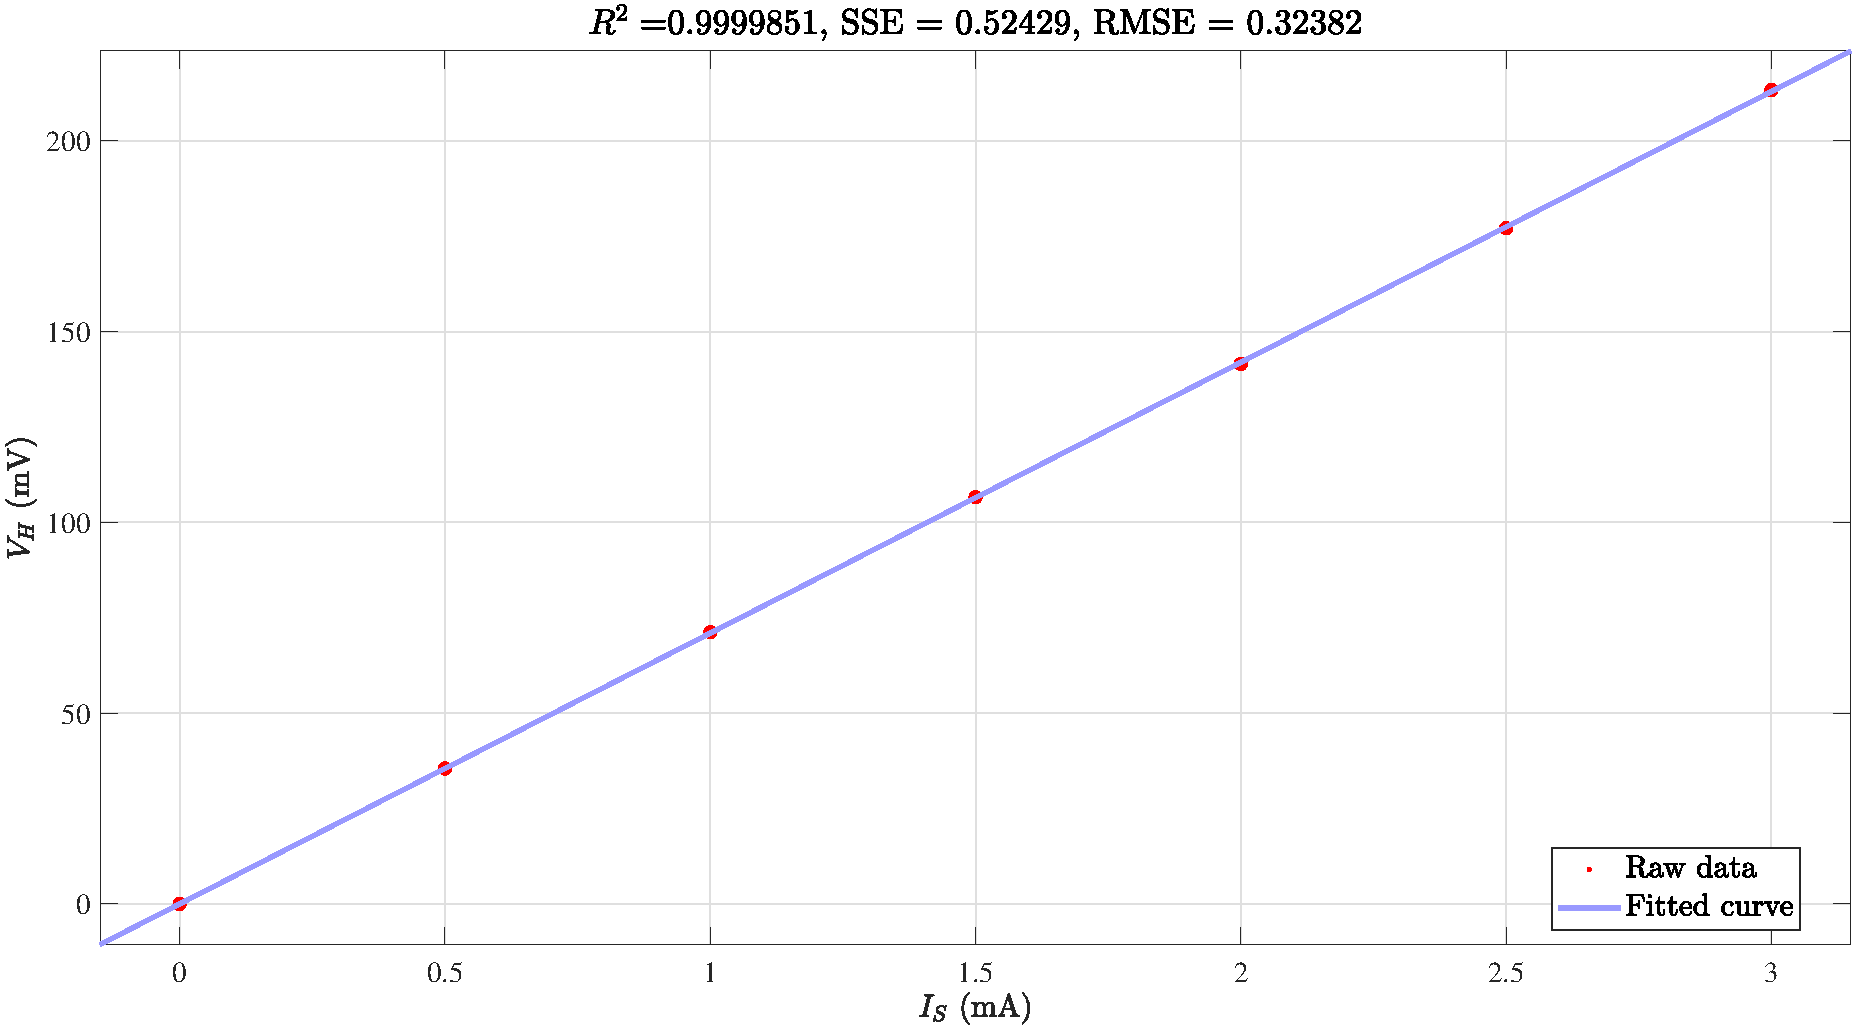
\includegraphics[scale=0.15]{1.jpg}
\end{figure}
\begin{figure}[H]
    \centering
    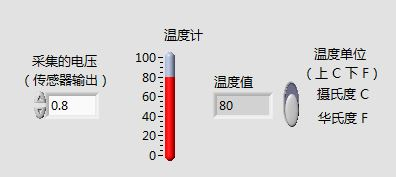
\includegraphics[scale=0.15]{3.jpg}
\end{figure}
\begin{figure}[H]
    \centering
    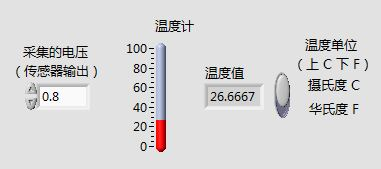
\includegraphics[scale=0.15]{2.jpg}
\end{figure}

$\quad$ \textbf{为什么积分常量会影响 $u_{R_1}-u_c$ 李萨如图形的形状?}\par
实验原理中,公式${u_C} = \frac{Q}{C} = \frac{1}{C}\int {{i_2}dt}  = \frac{1}{{C{R_2}}}\int {{u_{{R_2}}}dt}  \approx \frac{1}{{C{R_2}}}\int {{u_2}dt}$
的推导最后用的是约等于,而约等于
的条件是积分常数$R_2 C \gg T$,本实验频率 $f=100Hz$,即 $T=0.02s$,因此,在积分常数为 $0.5s$ 时,此
条件基本上满足,而变为 $0.05s$ 与$ 0.01s $时,该条件不再满足,因此会改变李萨如图形的形状

$\quad$\textbf{积分常量是否会影响真实的$ B − H $磁滞回线的形状?}\par
$u_c$的改变会影响$u_x$和$u_y$的比例,但$u_x$与$u_y$只影响到示波器上显示的图像,而真实的 $B − H $磁
滞回线的形状并不会因为示波器的显示而改变,故积分常量本质上对真实的磁滞回线并无影响。
\subsection{观测铁氧体的动态磁滞回线}
\begin{table}[H]
    \centering
    \caption{铁氧体的动态磁滞回线测量数据}
    \begin{tabular}{|l|l|l|l|l|l|l|l|l|l|l|}
    \hline
        ~ & 1 & 2 & 3 & 4 & 5 & 6 & 7 & 8 & 9 & 10\\ \hline
        H(A/m) & 22.5  & 24.23  & 27.12  & 29.42  & 31.73  & 38.08 & 38.65  & 41.54  & 50.19  & 66.92  \\ \hline
        B(T) & 0.67  & 0.75& 0.83  & 0.86  & 0.89  & 0.91  & 0.91  & 0.94  & 0.96  & 1  \\ \hline
        $\mu_m$(H/m) & 23768  & 24719  & 24456  & 23265  & 22247  & 19101  & 18816  & 18025  & 15897  & 16210  \\ \hline
       ~&11&12&13&14&15&16&17&18&19&20\\\hline
       H(A/m)&70.96&107.31&&&&&&&& \\\hline
       B(T)&1.1&1.13&&&&&&&&\\\hline
       $\mu_m$(H/m)&12360&8373&&&&&&&&\\\hline
    \end{tabular}
\end{table}

绘制图像:
\begin{figure}[H]
    \centering
    \includegraphics[scale=0.7]{图片2.png}
\end{figure}
\begin{figure}[H]
    \centering
    \includegraphics[scale=0.7]{图片3.png}
\end{figure}

可以估计得到铁氧体的起始磁导率大约为$12000H/m$

\subsection{观测硅钢的动态磁滞回线}
\begin{table}[H]
    \centering
    \begin{tabular}{|l|l|l|l|}
    \hline
        ~ & 20Hz & 40Hz & 60Hz \\ \hline
        $B_m$ & 0.97  & 0.91  & 0.94  \\ \hline
        $B_r$ & 0.54 & 0.59  & 0.7  \\ \hline
        $H_c$ & 62.3 & 73.85  & 80.77 \\ \hline
    \end{tabular}
\end{table}
观察比较三个频率下对应的数据,可以发现$B_m$,$B_r$的变化不大,在误差允许范围内可视作不变。
而$H_c$随着频率的增加而显著增大。

\subsection{测量铁氧体在不同直流偏置磁场下的可逆磁导率}
\begin{table}[H]
    \centering
    \caption{铁氧体在不同直流偏置磁场下的可逆磁导率}
    \begin{tabular}{|l|l|l|l|l|l|l|l|l|l|l|}
    \hline
        ~ & 1 & 2 & 3 & 4 & 5 & 6 & 7 & 8 & 9 & 10 \\ \hline
        电流(A) & 0.01 & 0.02 & 0.03 & 0.04 & 0.05 & 0.06 & 0.07 & 0.08 & 0.09 & 0.1 \\ \hline
        H(A/m) & 0.46  & 1.85  & 2.65  & 4.26  & 11.54  & 14.42  & 14.42  & 15.23  & 15.23  & 8.08  \\ \hline
        B(T) & 0.003  & 0.007  & 0.009  &0.009& 0.017& 0.015  & 0.013  & 0.009  & 0.007  & 0.002   \\ \hline
        $\mu_R$ & 5191  & 3152  & 2837  & 1764  & 1187  & 807  & 712 & 494  & 359  & 212 \\ \hline
    \end{tabular}
\end{table}

绘制图像:
\begin{figure}[H]
    \centering
    \includegraphics[scale=0.8]{图片4.png}
\end{figure}

通过观察图像可以发现,$u_R$随着H的增大而减小
\subsection{测量铁磁材料准静态磁滞回线}
\subsubsection{测量模具钢起始磁化曲线}
\begin{table}[H]
    \centering
    \caption{模具钢的起始磁化曲线数据}
    \begin{tabular}{|l|l|l|l|}
    \hline
        I(mA) & B(mT) & H(A/m) & 修正H(A/m) \\ \hline
        0 & 1.2 & 0.0  & -8.0  \\ \hline
        60.9 & 12.5 & 507.5  & 424.6  \\ \hline
        120.6 & 43.2 & 1005.0  & 718.5  \\ \hline
        180.6 & 80 & 1505.0  & 974.5  \\ \hline
        239.4 & 116.8 & 1995.0  & 1220.4  \\ \hline
        300.3 & 159.5 & 2502.5  & 1444.8  \\ \hline
        359.7 & 202.6 & 2997.5  & 1654.0  \\ \hline
        420.7 & 245.6 & 3505.8  & 1877.1  \\ \hline
        480.3 & 284.2 & 4002.5  & 2117.8  \\ \hline
        541.1 & 319.2 & 4509.2  & 2392.4  \\ \hline
        599.6 & 348.7 & 4996.7  & 2684.3 \\ \hline
    \end{tabular}
\end{table}

\begin{figure}[H]
    \centering
    \includegraphics[scale=0.9]{图片5.png}
\end{figure}

与理论曲线比较,实验所得图像与理论图像接近

\subsubsection{测量模具钢的磁滞回线}
\begin{figure}[H]
    \centering
    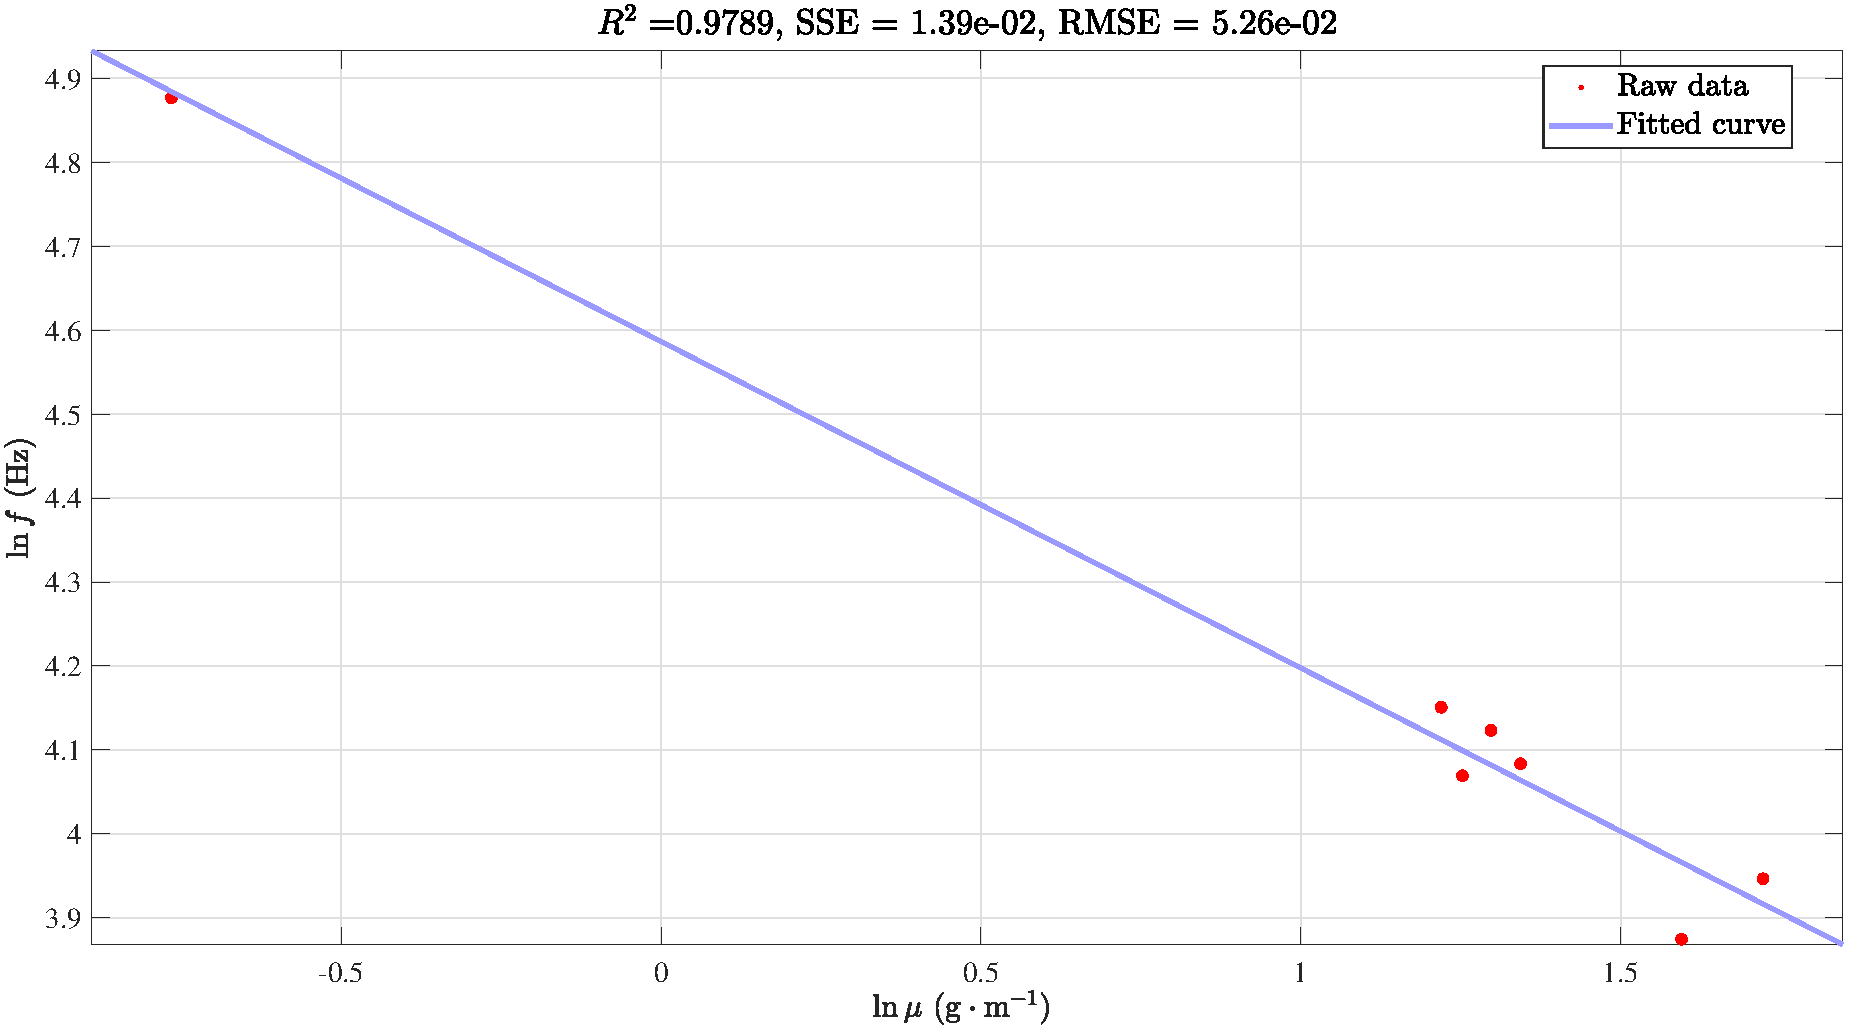
\includegraphics[scale=0.9]{5.png}
    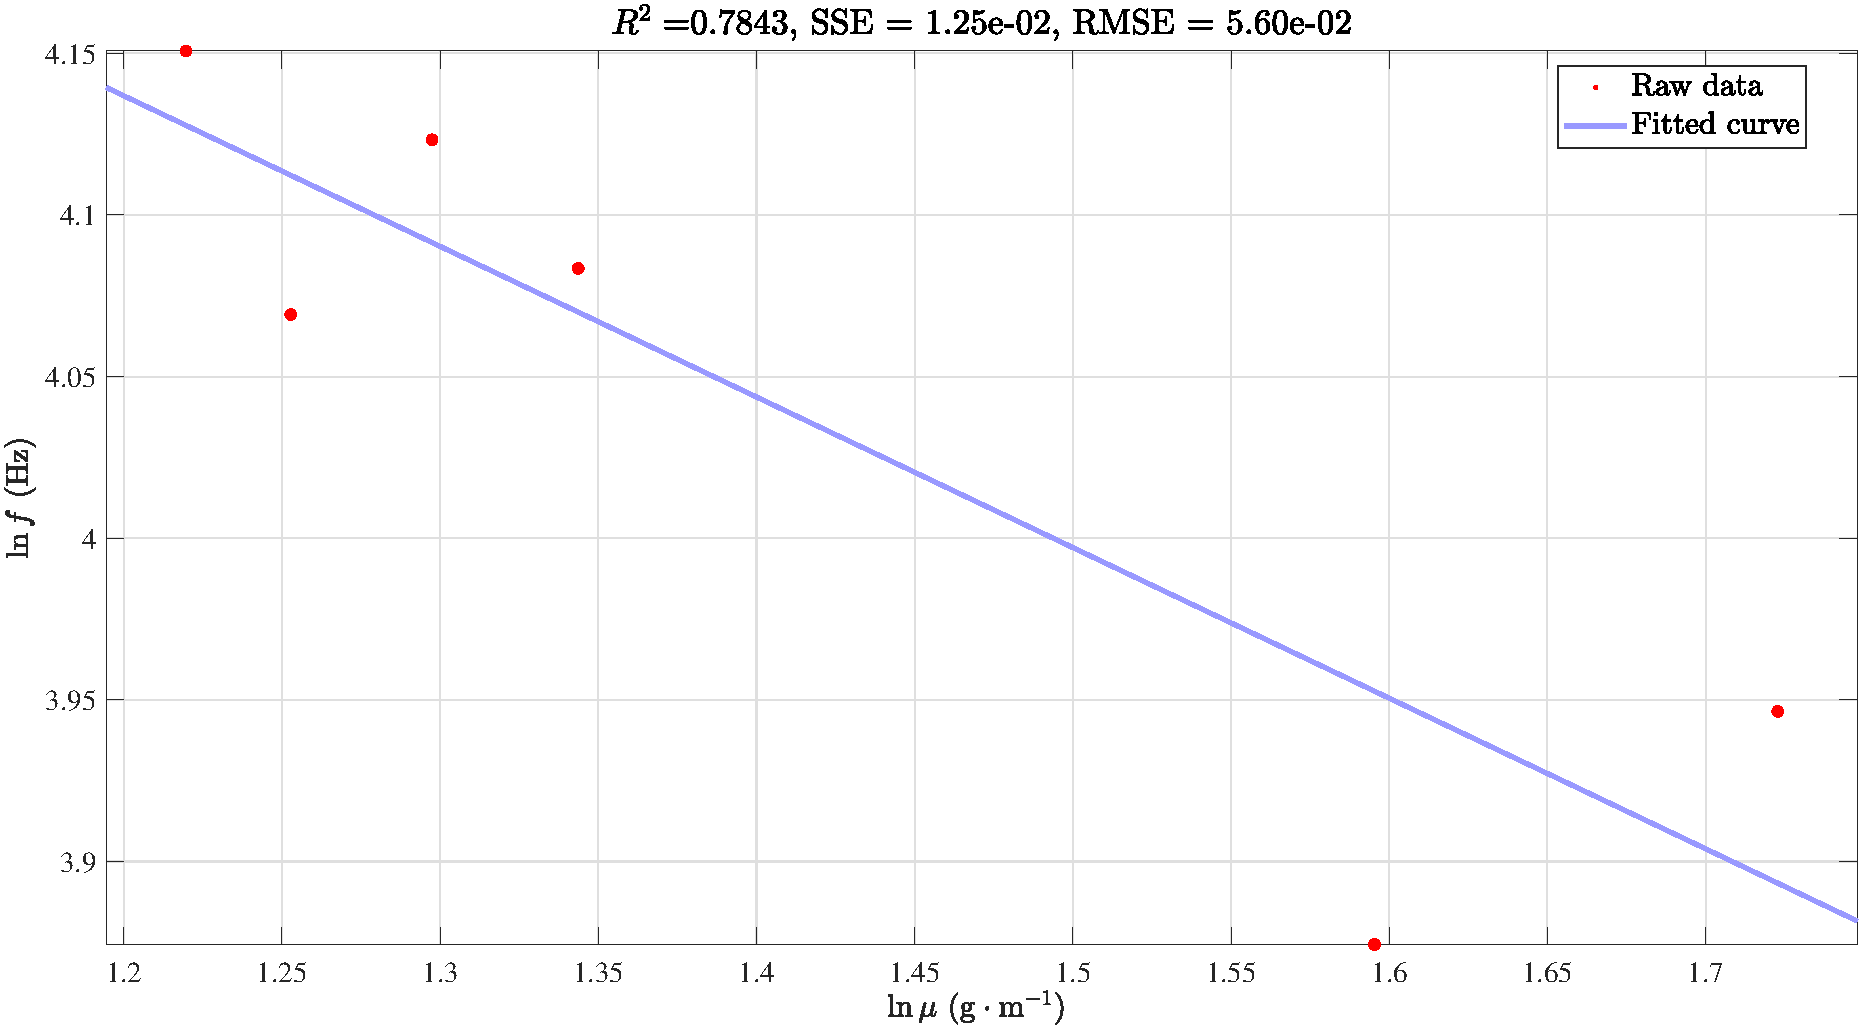
\includegraphics[scale=0.9]{6.png}
\end{figure}

绘制图像:
\begin{figure}[H]
    \centering
    \includegraphics[scale=0.9]{图片6.png}
\end{figure}

根据图像,可以看出硅钢的饱和磁感应强度约为$B_m=0.38(T)$,饱和磁场强度约为$2800(A/m)$,矫顽力
约为$H_c=800(A/m)$

但实验得到的图像与理论整体趋势一致,但是有明显的误差。这可能是由于磁锻炼不充分导致。实际实验
中,磁场和电流的读数均不稳定,存在由于读数引起的误差。

在开关拉动时,应该使触点从接触到断开的时间长一些,这会使得材料在当前磁场中磁化达到稳定。

\section{思考题}
    \subsubsection*{$\qquad1.$铁磁材料的动态磁滞回线与静态磁滞回线在概念上有什么区别?铁磁
    材料动态磁滞回线的形状和面积受哪些因素影响?}
        区别:动态磁滞回线是在交变电场的作用下得到的 B-H 关系曲线,静态磁滞回线是在材料磁化完全
    后,测量材料的 B-H 关系曲线。\par
        影响因素:动态磁滞回线受到铁磁材料种类、大小、交流电频率和振幅等多种因素的影响,其围成
    的面积等于一个周期的能量损耗,这些损耗除了磁滞损耗外,还包括涡流损耗与剩余损耗,这些也与铁
    磁材料种类、大小、交流电频率和振幅等有关,静态磁滞回线因为没有磁场大小随时间的变化,因此几
    乎没有涡流损耗和剩余损耗

    \subsubsection*{$\qquad2.$什么叫做基本磁化曲线?它和起始磁化曲线间有何区别?}
    基本磁化曲线指的是在磁场逐渐增加的过程中,铁磁材料磁化强度随着磁场的变化所呈现的曲线。
    而起始磁化曲线指的是在铁磁材料未经过磁化处理时,随着磁场的变化,其磁感应强度所呈现的曲线。
    两者的主要区别在于,基本磁化曲线是在经过磁化处理后才出现的,因此在磁化强度上会比起始磁化曲线高一些。

    此外,铁磁材料动态磁滞回线是描述材料在外加磁场下磁化强度随时间变化的曲线,其形状和面积受材料本身的磁性质、
    外加磁场的强度、频率和方向等因素的影响。而静态磁滞回线是描述材料在稳态下(即外加磁场恒定不变)的磁化强度和磁场的关系,
    其形状和面积主要受材料本身的磁性质影响。

    \subsubsection*{$\qquad3.$铁氧体和硅钢材料的动态磁化特性各有什么特点?}
    铁氧体的饱和磁感应强度一般较低。在高频磁场作用下,铁氧体材料的动态磁滞损耗较小。铁氧体材料的磁导率较高,硅钢材料的磁导率较低。

    \subsubsection*{$\qquad4.$动态磁滞回线测量实验中,电路参量应怎样设置才能保$u_{R_1}-u_C$所形成的李萨如图形正确反映材料动态磁滞回线的形状?}
    时间积分常数要满足$R_2 C\gg T$,才能使用推导中的近似公式,使得示波器中的图形可以反映动态磁滞
回线的形状。

    \subsubsection*{$\qquad5.$准静态磁滞回线测量实验中,为什么要对样品进行磁锻炼才能获得稳定的饱和磁滞回线?}
    磁锻炼会使材料的 B-H 关系不断接近饱和状态下的理论曲线,最终得到较为稳定的磁滞回线。
\section{实验总结与反思}
1.本次实验中,使用示波器进行测量误差较大,原因是实验使用的示波器无法自动得出所需的电压值,需要人工肉眼调试,容易出现差错

2.在判断磁滞回线是否饱和时,存在较大的主观因素。

3.实验采集数据点过少,尤其测量铁氧体的动态磁化曲线时,绘图时误差较大

\section*{附:原始实验数据}
\begin{figure}[H]
    \centering
    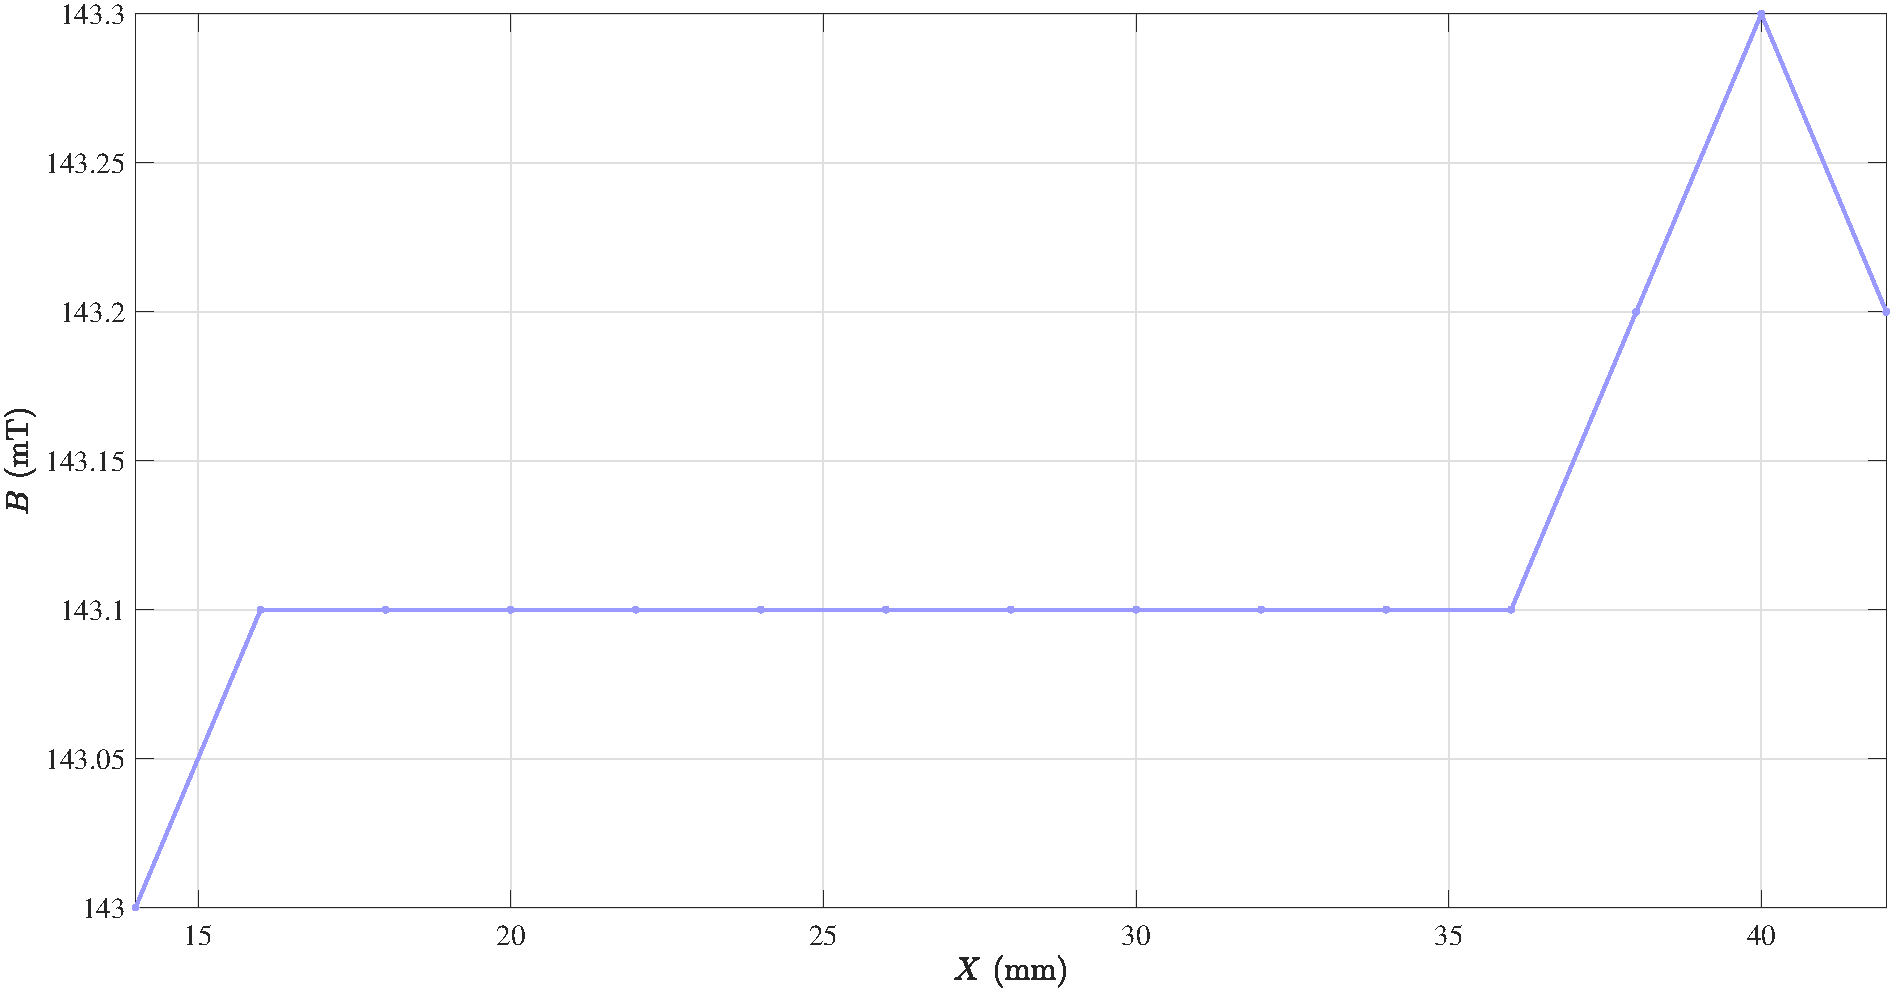
\includegraphics[scale=0.15]{4.jpg}
\end{figure}
\begin{figure}[H]
    \centering
    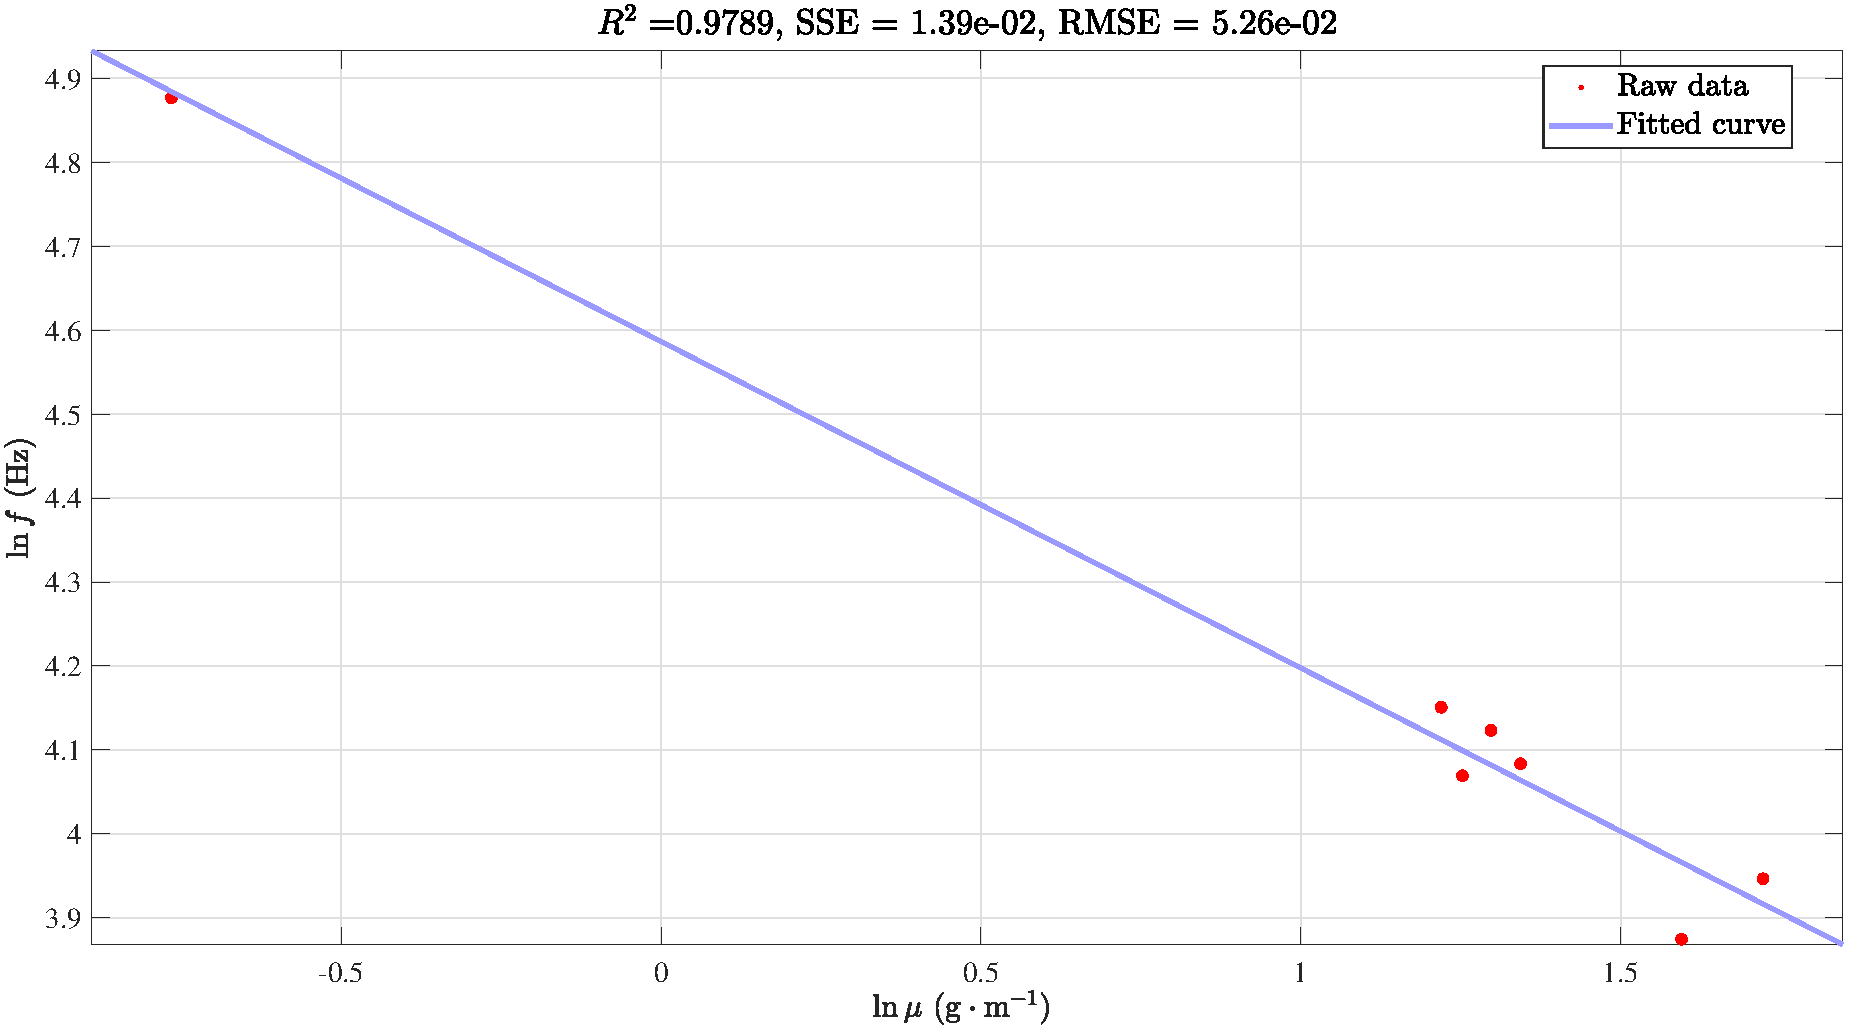
\includegraphics[scale=0.15]{5.jpg}
\end{figure}
\begin{figure}[H]
    \centering
    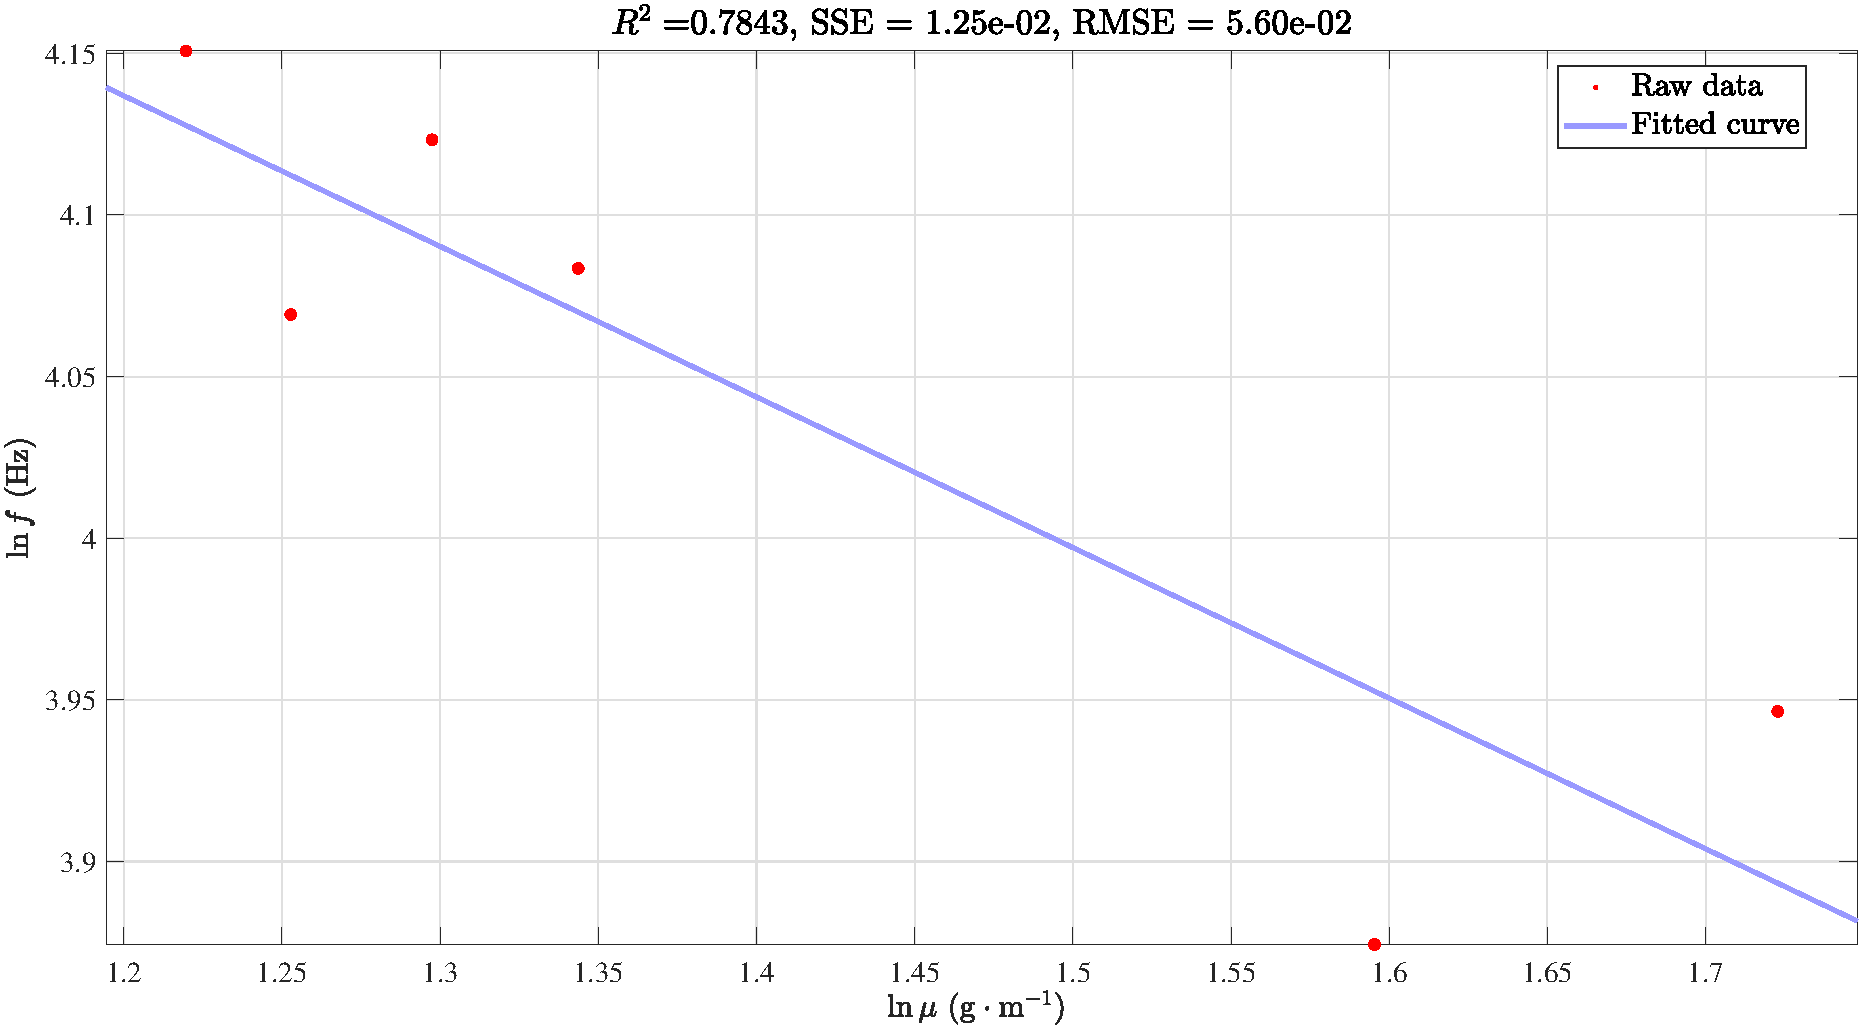
\includegraphics[scale=0.15]{6.jpg}
\end{figure}
\begin{figure}[H]
    \centering
    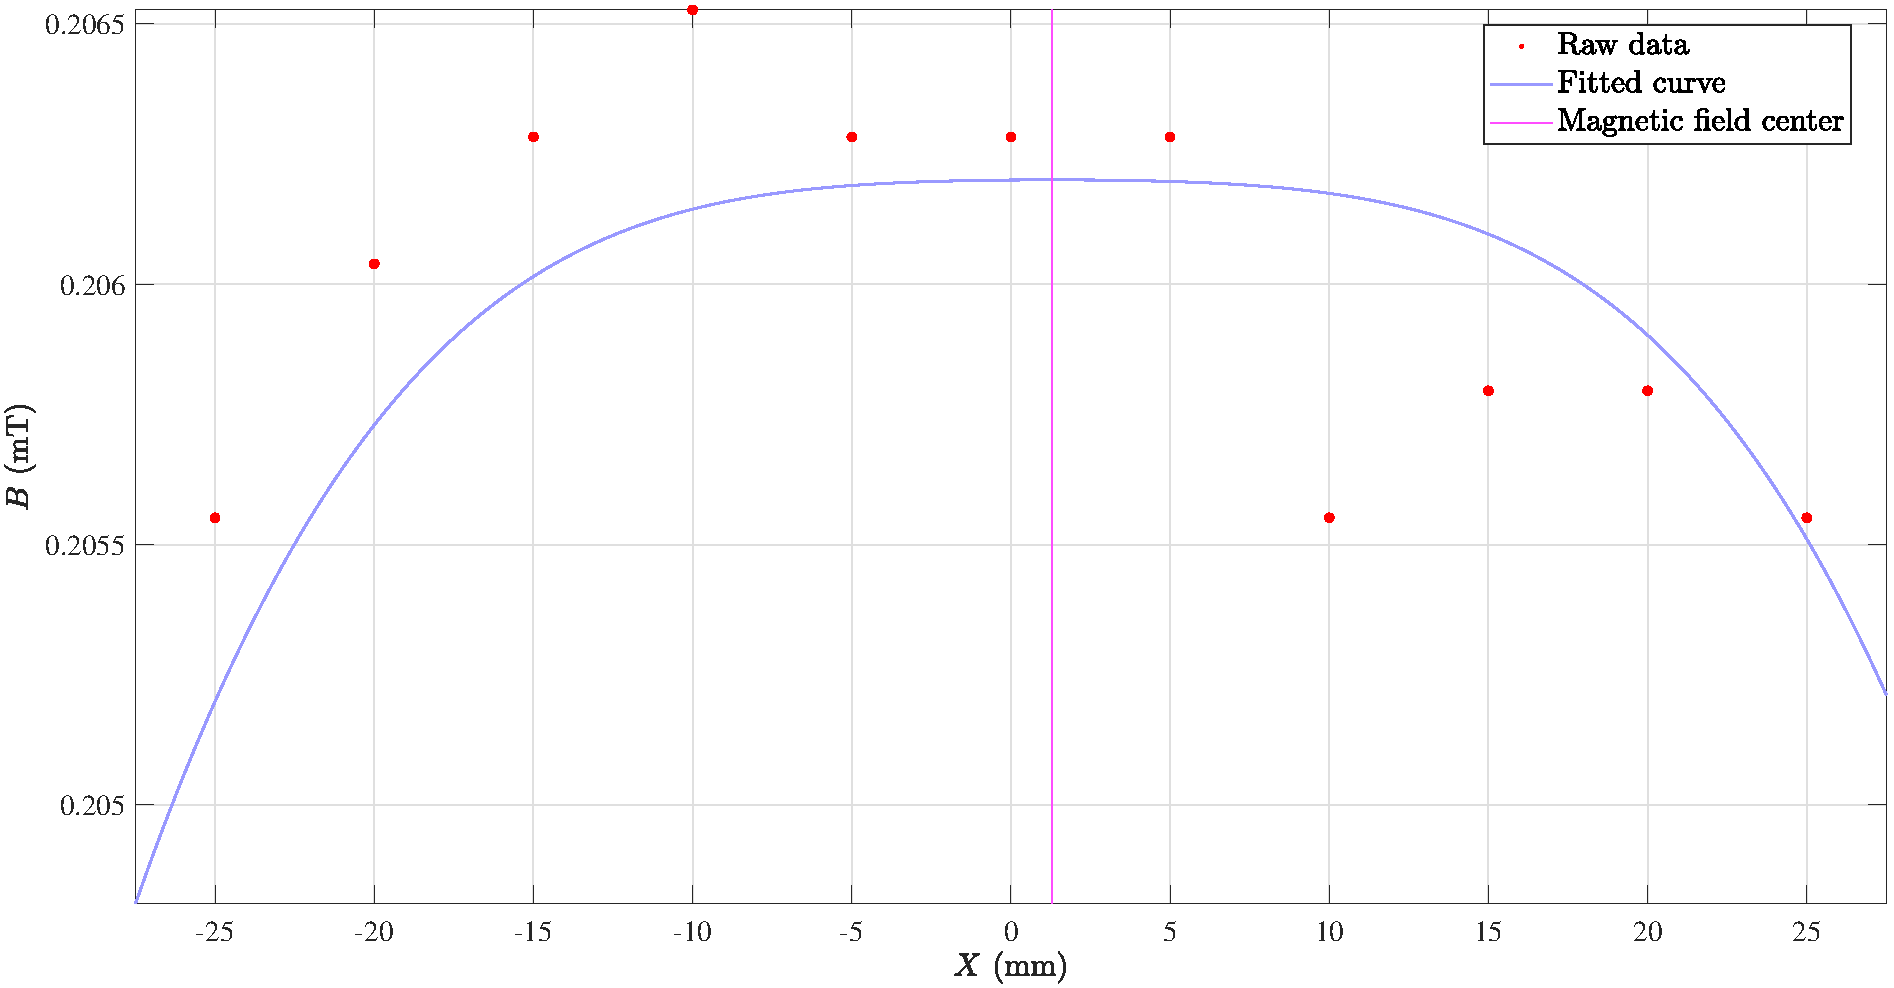
\includegraphics[scale=0.15]{7.jpg}
\end{figure}
\begin{figure}[H]
    \centering
    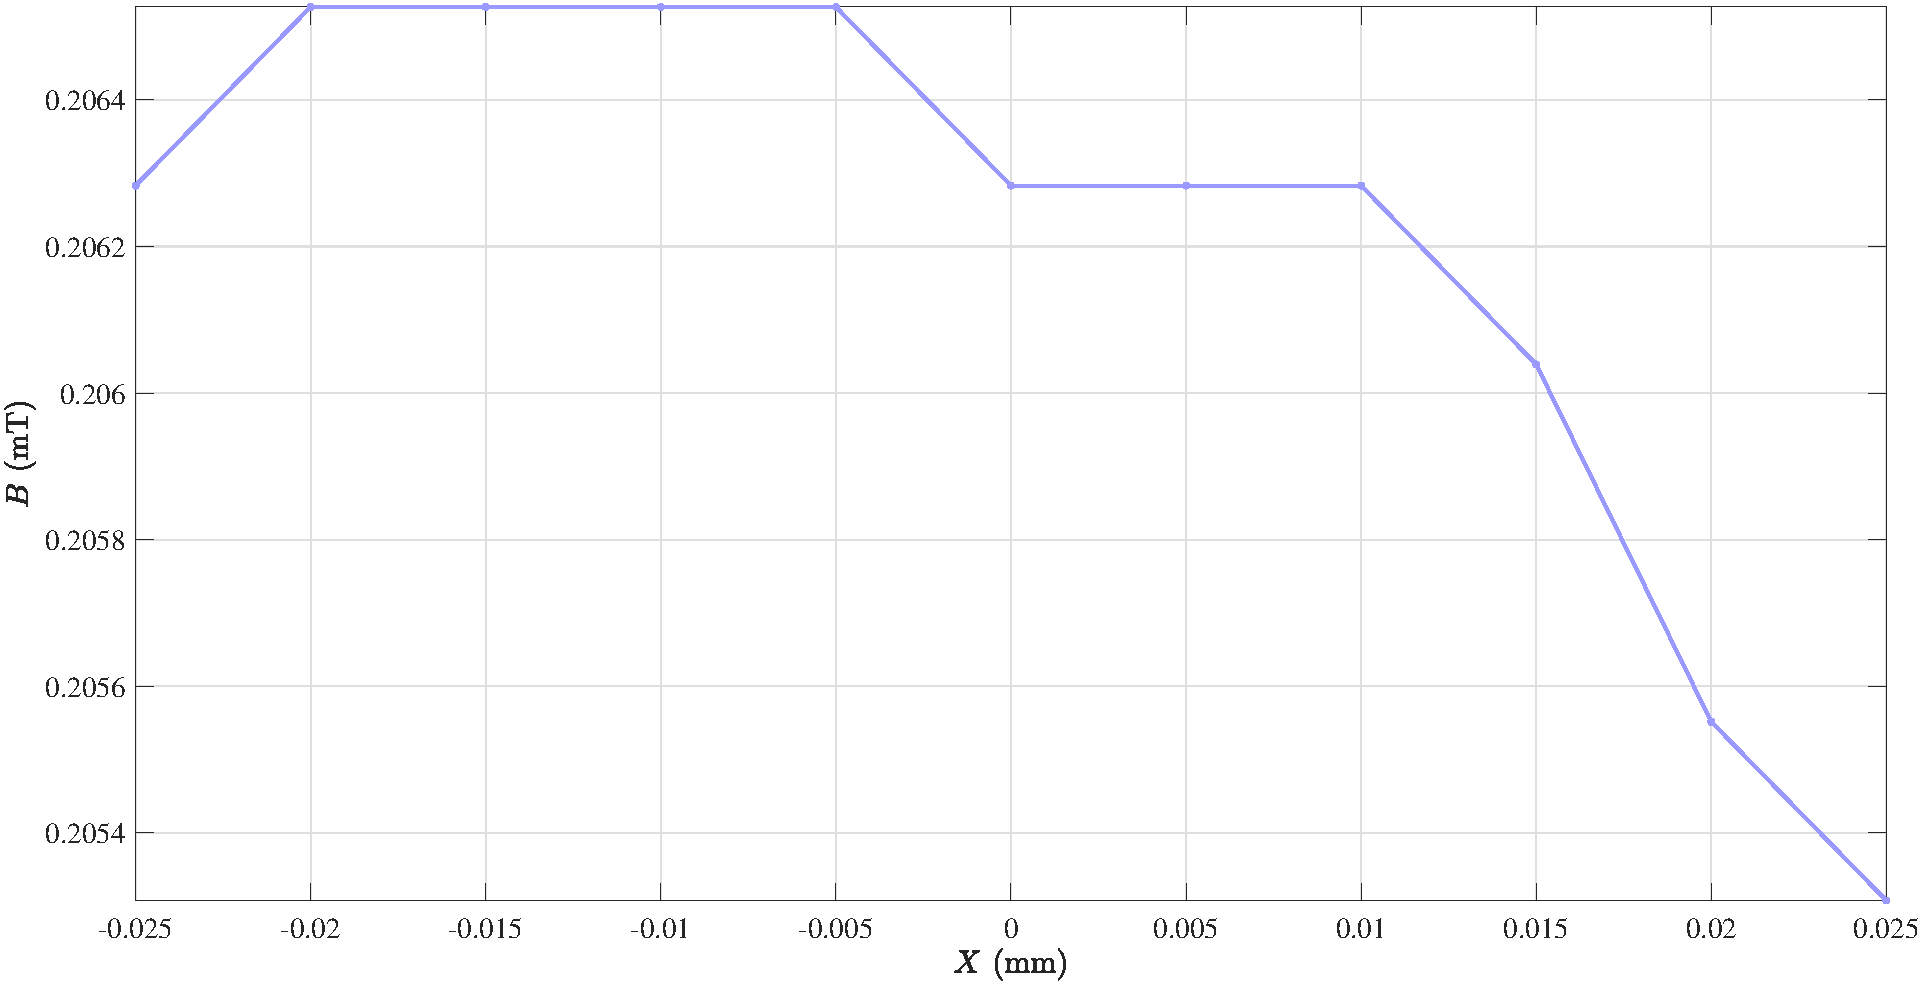
\includegraphics[scale=0.15]{8.jpg}
\end{figure}
\end{document}
